The Matlab code used to generate the plots is shown below.
\begin{lstlisting}
% transfer functions for plants and controllers
P_in = tf([b0],[1,0,0]);
P_out = tf(-P.g,[1,0,0]);
C_in = tf([(P.kd_th+P.sigma*P.kp_th), P.kp_th], [P.sigma, 1]);
C_out = tf([(P.kd_z+P.kp_z*P.sigma),...
            (P.kp_z+P.ki_z*P.sigma),P.ki_z],[P.sigma,1,0]);

% margin and bode plots 
figure(1), clf, margin(P_in*C_in), grid on, hold on
bode(P_in*C_in/(1+P_in*C_in)) 
margin(P_out*C_out)
bode(P_out*C_out/(1+P_out*C_out))
legend('Open Loop-Inner', 'Closed Loop-Inner',...
       'Open Loop-Outer', 'Closed Loop-Outer')
\end{lstlisting}

The transfer functions for the inner and outer loop plants and controller are defined in Lines~2--6.  For this problem we plot both the inner and outer loop frequency response on the same Bode plot, as implemented in Lines~9--14. The results of this code are shown in Figure~\ref{fig:hw_ballbeam_margins}.
\begin{figure}[H]
   \centering
   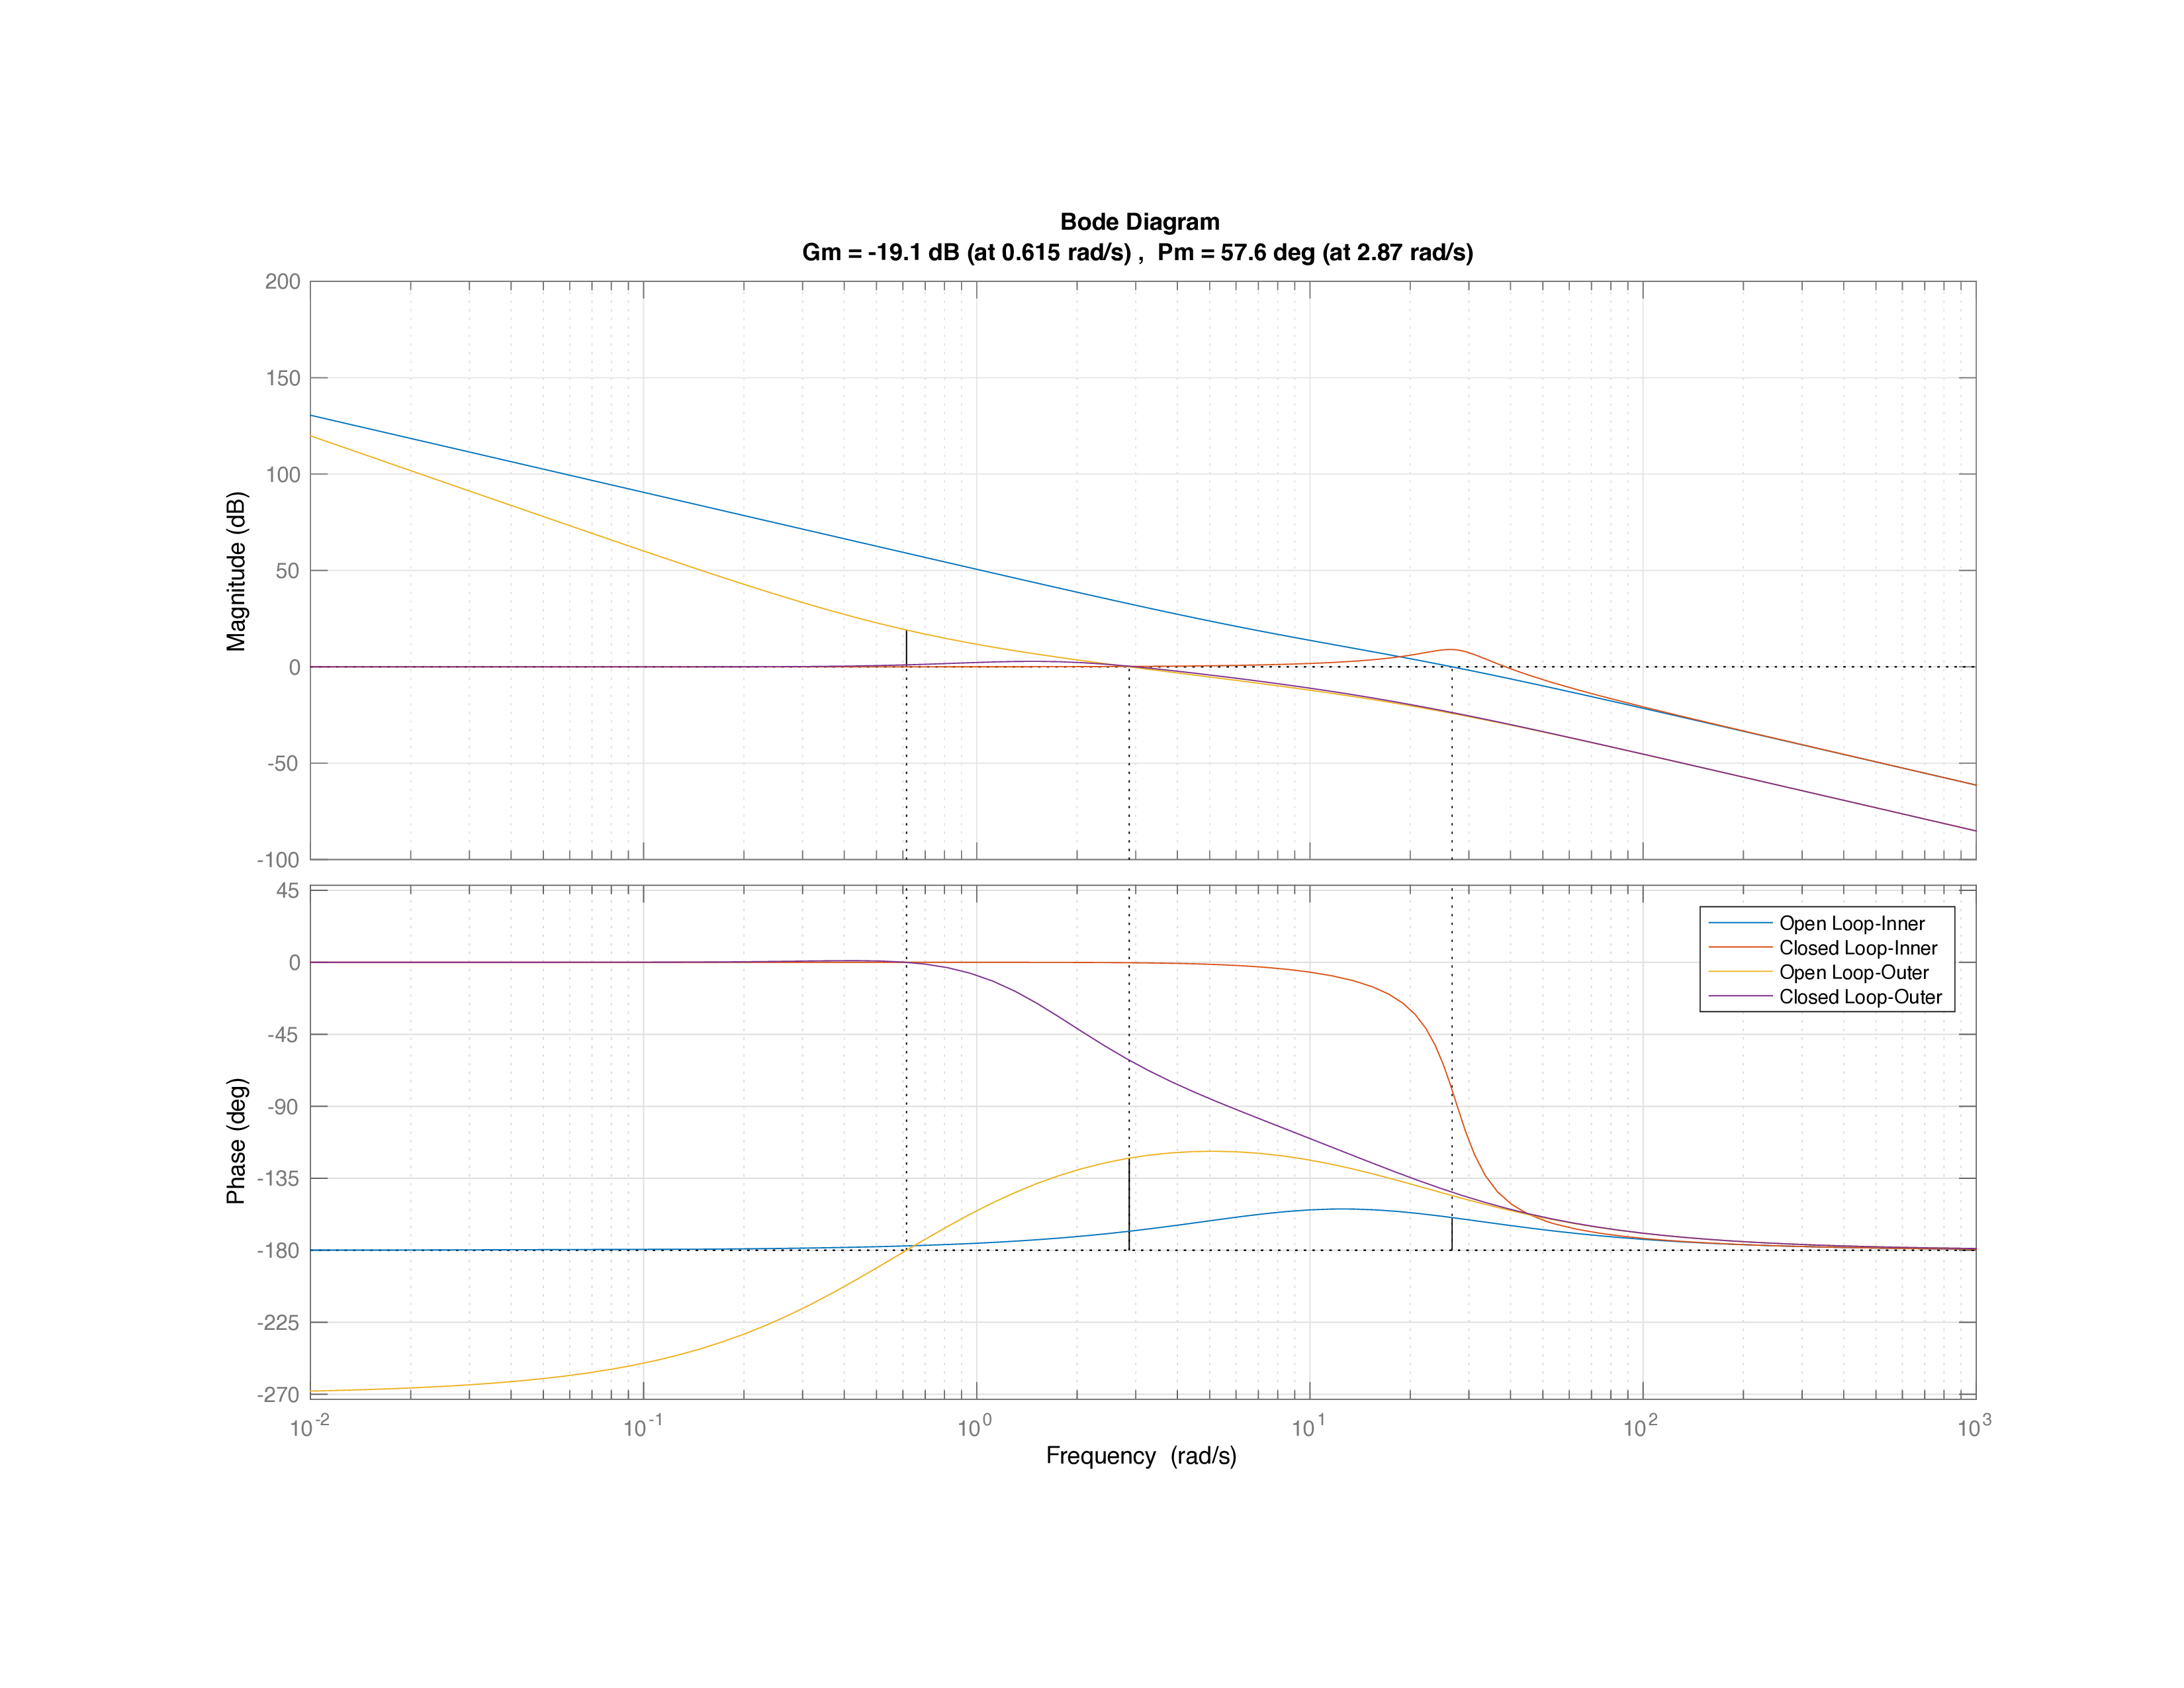
\includegraphics[width=0.95\textwidth]{6_design_studies/figures/hw_ballbeam_margins.pdf}
   \caption{The {\tt margin} and {\tt bode} plots for the the open and closed loop systems of both the inner and outer loops of the ballbeam system.}
   \label{fig:hw_ballbeam_margins}
\end{figure} 
As seen from Figure~\ref{fig:hw_ballbeam_margins} the bandwidth of the inner loop is approximately $44$~rad/sec, which is 1.7 times larger than the cross over frequency of $26$~rad/sec.  The larger bandwidth is due to the small phase margin of $PM=20$~degrees.
%
Similarly, Figure~\ref{fig:hw_ballbeam_margins} indicates that the bandwidth of the outer loop is $4.2$~rad/sec, which is 1.5 times larger than the cross over frequency of $2.8$~rad/sec.  The higher phase margin of $PM=58$~degrees increases the damping in the system and lowers the bandwidth slightly.
%
The closed-loop magnitude for the inner loop is approximately one at frequencies up to five times the bandwidth of the inner loop. Furthermore, the phase of the closed inner loop system is near zero up to frequencies above the crossover frequency of the outer loop. This bandwidth separation ensures that the influence of the inner loop on the outer loop design and operation is minimal within the bandwidth of the inner loop.